\section{Auswertung}
\label{sec:Auswertung}

Alle in der Auswertung benutzten Mittelwerte werden mithilfe der Gleichung
\begin{equation}
\tilde{x}=\frac{1}{n}\sum_{i=1}^n {x_i}
\end{equation}
bestimmt. Die Standardabweichungen der Mittelwerte ergeben sich mit der Formel
\begin{equation}
\mathup\Delta{\tilde{x}}=\sqrt{\frac{1}{n(n-1)}\sum_{i=1}^n {(x_i-\tilde{x})²}}.
\end{equation}
Wird eine Größe beziffert, welche sich aus fehlerbehafteten Daten zusammensetzt, wird der absolute Fehler über die Gaußsche Fehlerfortpflanzung erhalten.
Hierzu gilt
\begin{equation}
\mathup\Delta{f}(x_1,..,x_n)=\sqrt{\left(\frac{\mathup{d}f}{\mathup{d}x_1}\Delta{x_1}\right)²+..+\left(\frac{\mathup{d}f}{\mathup{d}x_n}\Delta{x_n}\right)²}.
\end{equation}
Zur Berechnung aller Größen werden rechnerintern nicht-gerundete Größen mit maximaler Anzahl der Nachkommastellen benützt.
Die angegeben Werte werden auf die erste signifikante Stelle des Fehlers gerundet.

\subsection{Bestimmung der Hintergrundstrahlung und statistische Betrachtung}
\label{sec:Auswertung_hintergrund}
Die statische Verteilung der Zerfälle sowie die natürlich auftretende Strahlung nehmen Einfluss auf die Zuverlässigkeit der Messwerte.
Um genaue statistische Aussage treffen zu können, werden die im Zeitintervall $\mathup\Delta t$ detektierten Zerfälle $\mathup\Delta N$ gemäß
\begin{equation}
	n=\frac{\mathup\Delta N}{\mathup\Delta t}
\end{equation}
bestimmt.
Die Fehler werden anders als im Auswertungspräambel nicht durch wiederholte Messung bestimmt, sondern mit
\begin{equation}
	\mathup\Delta n=\frac{\sqrt{\mathup\Delta N}}{\mathup\Delta t}
\end{equation}
als gegeben angenommen.
Von den Messungen wird die im Voraus gemessene Hintergrundstrahlung abgezogen. 
Für diese gilt im Folgenden
\begin{equation}
	n_0=\frac{166}{\SI{900}{\second}}\approx\SI{0.18(1)}{\hertz},
	%=\frac{\mathup\Delta N}{\mathup\Delta t}=
\end{equation}
das Herausrechnen der Hintergrundstrahlung bei Messwert $N_\text{Messung}$, welche im Zeitintervall $\mathup\Delta t$ aufgenommen wurde, folgt der Formel
\begin{equation}
	N=N_{\text{Messung}}-N_0\cdot\mathup\Delta t.
\end{equation}

\subsection{Zerfallsgesetz}
Der radioaktiver Zerfall wird durch exponentiellen Abfall beschrieben.
Hierfür gilt in guter Näherung
\begin{equation}
	N(t)=N_0 \exp(-\lambda t),
	\label{eq:Zerfallsgesetz}
\end{equation}
welches beim Auftrag mit halblogarithmischer Skalierung eine lineare Regression,
\begin{equation}
	\ln(N(t))=\ln(N_0(\exp(-\lambda t))=\ln(N_0)+\ln(\exp(-\lambda t)) =\underbrace{\ln(N_0)}_{A_\text{Reg}}-\underbrace{\lambda}_{m_\text{Reg}} \cdot t,
	\label{eq:Zerfallsgesetz_linear}
\end{equation}
zulässt.
Charakteristische Größe bei der Betrachtung von Zerfällen ist die Halbwertzeit \ref{sec:Theorie}, Gleichung \eqref{eq:halbwertszeit}, die mit der Zerfallskonstante $\lambda$ in Verbindung steht.

\subsection{Messung von Indium}
In Tabelle \ref{tab:indium} sind die Messwerte $N_\text{Messung}$, deren korrigierte Werte $N$ und der Messzeitpunkt $t$ abgebildet.
\begin{table}[htp]
	\centering
		\begin{tabular}{S[table-format=4.0]
                        S[table-format=4.0]
                        S}
			\toprule
			{$t\,\text{in}\,\si{\second}$} & {$N_\text{Messung}$} & {$N$}\\
			\midrule
			 250 & 2038 &  2000(40)\\
			 500 & 1994 &  1950(40)\\
			 750 & 1867 &  1820(40)\\
			1000 & 1740 &  1700(40)\\
			1250 & 1611 &  1560(40)\\
			1500 & 1608 &  1560(40)\\
			1750 & 1473 &  1430(40)\\
			2000 & 1415 &  1370(30)\\
			2250 & 1311 &  1260(30)\\
			2500 & 1234 &  1190(30)\\
			2750 & 1213 &  1170(30)\\
			3000 & 1200 &  1150(30)\\
			3250 & 1055 &  1010(30)\\
			3500 &  971 &   920(30)\\
			3750 &  901 &   850(30)\\
			\bottomrule
		\end{tabular}
	\caption{Messwerte: Zerfälle bei der Messung von Indium beim Zeitintervall von \SI{250}{\second}.}
	\label{tab:indium}
\end{table}
\begin{figure}[h]
    \centering
    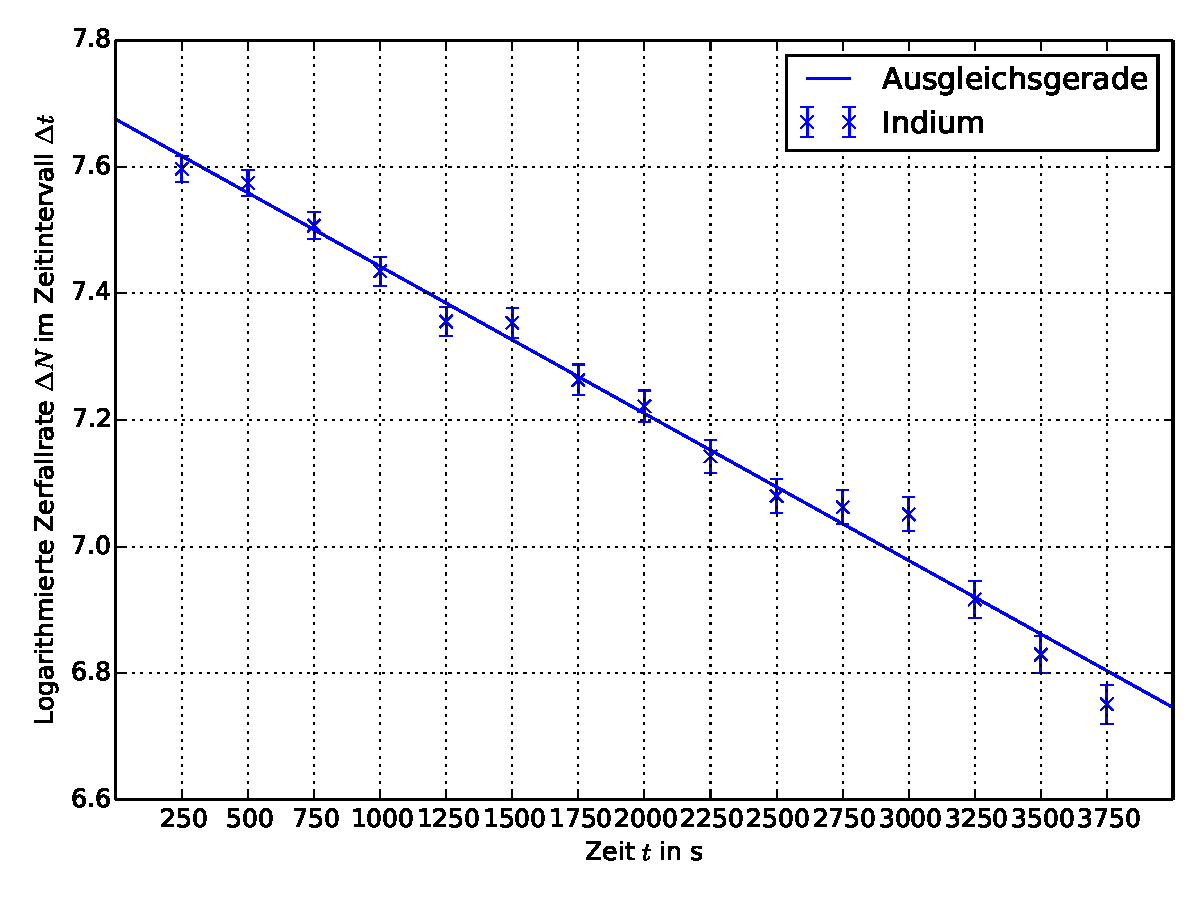
\includegraphics[width=\textwidth]{Bilder/indium.pdf}
    \caption{Korrigierte und logarithmierte Anzahl der Zerfälle für Indium aufgetragen gegen die Zeit.}
    \label{fig:indium}
\end{figure}

In Abbildung \ref{fig:indium} sind die Zerfälle $N$ pro Zeit gegen die fortschreitende Zeit aufgetragen.
Die Messwerte sind gemäß der Überlegung im vorangegangenen Abschnitt logarithmiert, die Skaleneinteilung verbleibt daher linear.


\subsection{Messung von Rhodium}
In Tabelle \ref{tab:rhodium} sind die Messwerte $N_\text{Messung}$, deren korrigierte Werte $N$ und der Messzeitpunkt $t$ abgebildet.
\begin{table}[htp]
	\centering
		\begin{tabular}{S[table-format=2.0]
                        S[table-format=3.0]
                        S}
			\toprule
			{$t\,\text{in}\,\si{\second}$} & {$N_\text{Messung}$} & {$N$}\\
			\midrule
				20	&	545	&540(20)\\
				40	&	392	&390(20)\\
				60	&	329	&330(20)\\
				80	&	238	&230(20)\\
				100	&	221	&220(20)\\
				120	&	178	&170(10)\\
				140	&	122	&120(10)\\
				160	&	112	&110(10)\\
				180	&	 90	&86(9)\\
				200	&	 72	&68(8)\\
				220	&	 54	&50(7)\\
				240	&	 71	&67(8)\\
				260	&	 40	&36(6)\\
				280	&	 51	&47(7)\\
				300	&	 35	&31(6)\\
				320	&	 34	&30(6)\\
				340	&	 38	&34(6)\\
				360	&	 28	&24(5)\\
				380	&	 34	&30(6)\\
				400	&	 22	&18(4)\\
				420	&	 26	&22(5)\\
				440	&	 20	&16(4)\\
				460	&	 19	&15(4)\\
				480	&	 22	&18(4)\\
				500	&	 14	&10(3)\\
				520	&	 19	&15(4)\\
				540	&	 21	&17(4)\\
				560	&	 15	&11(4)\\
				580	&	 20	&16(4)\\
				600	&	 23	&19(5)\\
				620	&	 18	&14(3)\\
				640	&	 24	&20(5)\\
				660	&	 11	&7(3)\\
				680	&	 13	&9(3)\\
				700	&	 19	&15(4)\\
				720	&	 11	&7(3)\\
				740	&	 15	&11(4)\\
				760	&	 14	&10(3)\\
				780	&	 18	&14(4)\\
				800	&	 13	&9(3)\\
			\bottomrule
		\end{tabular}
	\caption{Messwerte: Zerfälle bei der Messung von Rhodium beim Zeitintervall von \SI{20}{\second}.}
	\label{tab:rhodium}
\end{table}
\begin{figure}[h]
    \centering
    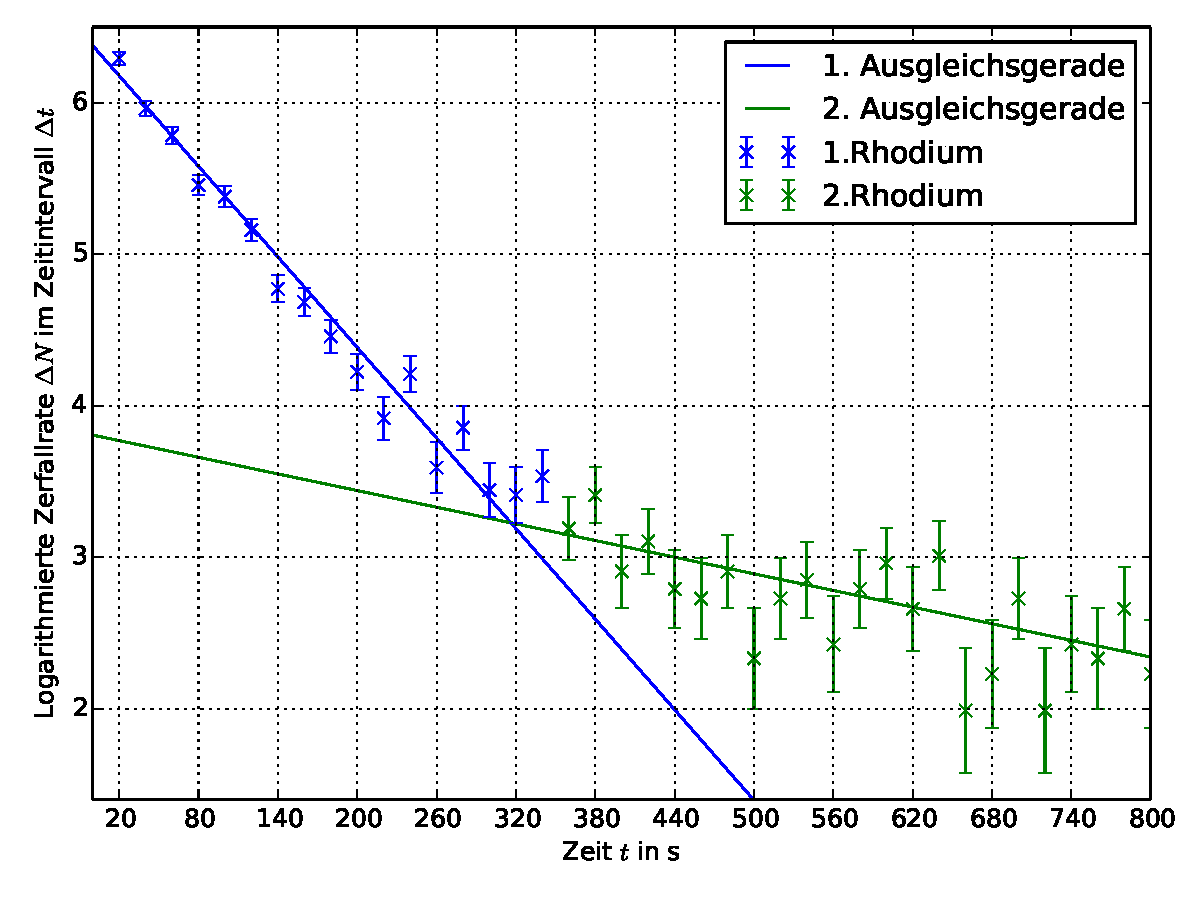
\includegraphics[width=\textwidth]{Bilder/rhodium.pdf}
    \caption{Korrigierte und logarithmierte Anzahl der Zerfälle für Rhodium aufgetragen gegen die Zeit.}
    \label{fig:rhodium}
\end{figure}